  \documentclass[a4]{beamer}
\usepackage{amssymb}
\usepackage{graphicx}
\usepackage{subfigure}
\usepackage{newlfont}
\usepackage{amsmath,amsthm,amsfonts}
%\usepackage{beamerthemesplit}
\usepackage{pgf,pgfarrows,pgfnodes,pgfautomata,pgfheaps,pgfshade}
\usepackage{mathptmx} % Font Family
\usepackage{helvet} % Font Family
\usepackage{color}
\mode<presentation> {
\usetheme{Frankfurt} % was Frankfurt
\useinnertheme{rounded}
\useoutertheme{infolines}
\usefonttheme{serif}
%\usecolortheme{wolverine}
% \usecolortheme{rose}
\usefonttheme{structurebold}
}
\setbeamercovered{dynamic}
\title[MA4413]{Statistics for Computing \\ {\normalsize MA4413 Lecture 5A}}
\author[Kevin O'Brien]{Kevin O'Brien \\ {\scriptsize kevin.obrien@ul.ie}}
\date{Autumn 2012}
\institute[Maths \& Stats]{Dept. of Mathematics \& Statistics, \\ University \textit{of} Limerick}
\renewcommand{\arraystretch}{1.5}
\begin{document}

%----------------------------------------------------------------------------------------------------%
\frame{
\frametitle{Continuous Random Variable} 
A continuous random variable is one which takes an infinite number of possible values. Continuous random variables are usually measurements. Examples include height, weight, the amount of sugar in an orange, the time required to run a mile.
\\
\bigskip
In this module, we will look at random variables from the following distributions
\begin{itemize}
\item Continuous uniform probability distribution
\item Exponential probabilty distribution
\item Normal probability distribution
\end{itemize}

Before this, we will look at some important concepts.
}


\begin{frame}
\frametitle{Continuous Random variables}
\begin{itemize}
\item Previously we have been studying discrete random variables, such as the Binomial and the Poisson random variables.
\item Now we turn our attention to continuous random variables.
\item Recall that a continuous random variable is one which takes an infinite number of possible values, rather than just a countable number of distinct values.
\item Continuous random variables are usually measurements.
\item Examples include height, weight, the amount of sugar in an orange, the time required to run a mile.
\end{itemize}
\end{frame}
%------------------------------------------------------------------%
\frame{
\frametitle{Exact Probabilities}
\large
\alert{Remarks:} This is for continuous distributions only.
\begin{itemize}
\item The probability that a continuous random variable will take an exact value is infinitely small.
We will usually treat it as if it was zero.
\item
When we write probabilities for continuous random variables in mathematical notation, we often retain the equality component (i.e. the "...or equal to..").\\
For example, we would write expressions $P(X \leq 2)$ or $P(X \geq 5)$.
\item
Because the probability of an exact value is almost zero, these two expression are equivalent to $P(X < 2)$
or $P(X > 5)$. \item The complement of $P(X \geq k)$ can be written as $P(X \leq k)$.
\end{itemize}
}
%----------------------------------------------------------------------------------------------------%
\begin{frame}
\frametitle{Functions and Definite integrals}
\begin{itemize}
\item Integration is not part of the syllabus, and it is assumed that students have are not familiar with how to compute definite integrals.
\item However,  it is useful to know what the purpose of definite integrals are, because we will be using the results derived from definite integrals. \item It is assumed that students are familiar with functions.
\end{itemize}
\end{frame}
%----------------------------------------------------------------------------------------------------%
\begin{frame}
\frametitle{Functions}

\vspace{-0.5cm}

\begin{center}
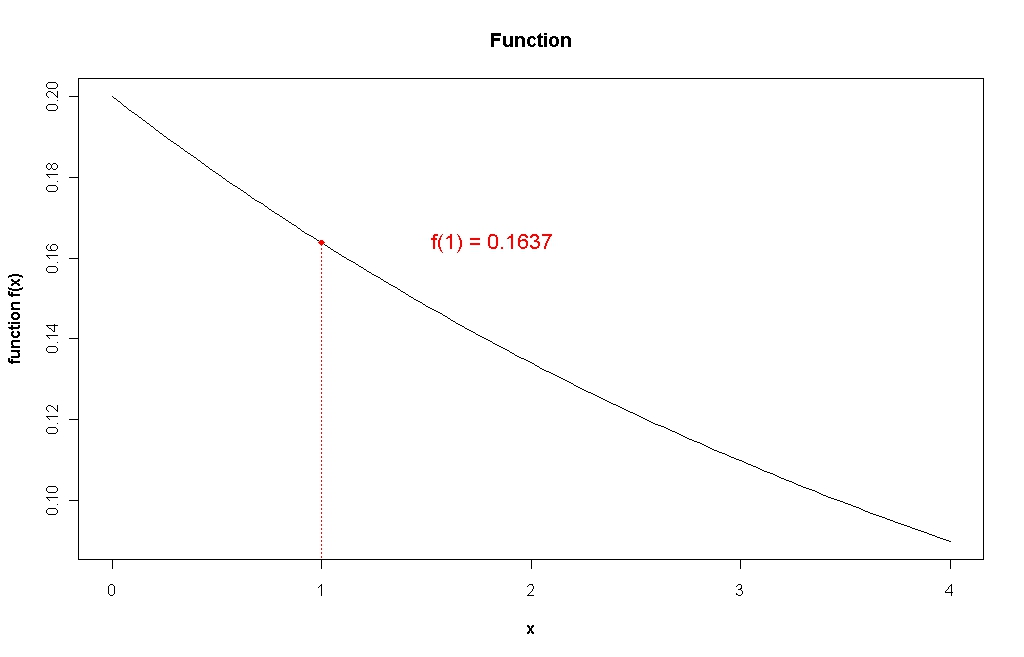
\includegraphics[scale=0.30]{images/6AFunction}

\end{center}

Some function $f(x)$ evaluated at $x=1$.
\end{frame}
%----------------------------------------------------------------------------------------------------%
\begin{frame}
\frametitle{Definite Integral}

\vspace{-0.5cm}
\begin{center}
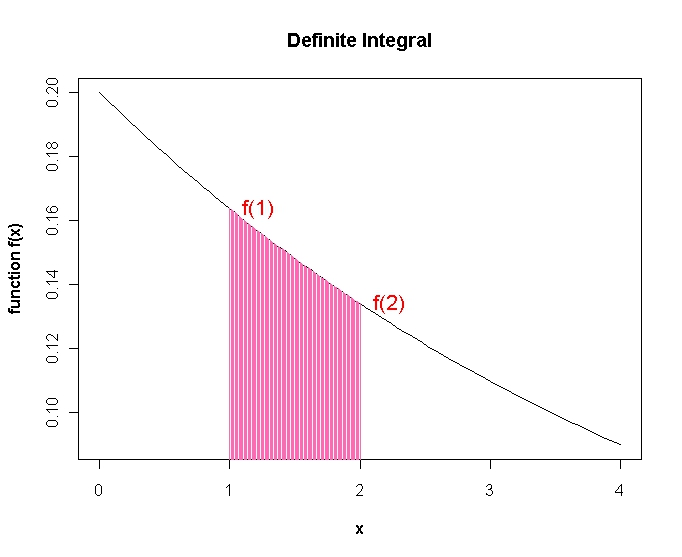
\includegraphics[scale=0.35]{images/6ADefiniteIntegral}
\end{center}
Definite integral of function is area under curve between X=1 and X=2.
\end{frame}

%----------------------------------------------------------------------------------------------------%
\begin{frame}
\frametitle{Definite Integral}

Definite integrals are used to compute the "area under curves". 

The area under the curve between X=1 and  X=2 is depicted in grey. Using definite integrals

\end{frame}
%----------------------------------------------------------------------------------------------------%
\begin{frame}
\frametitle{Definite Integral}
\begin{itemize}
\item Definite integrals are used to compute the ``area under curves".
\item Definite integrals are defined by a lower and upper limit.
\item The area under the curve between X=1 and  X=2 is depicted in the previous slide.
\item By computing the definite integral, we are able to determine a value for this area.
\item Probability can be represented as an area under a curve.
\end{itemize}
\end{frame}

%----------------------------------------------------------------------------------------------------%
\frame{

\frametitle{Probability Density Function}
\begin{itemize}
\item
In probability theory, a \textbf{\emph{probability density function}} (PDF) (or ``density" for short ) of a continuous random variable is a function that describes the relative likelihood for this random variable to occur at a given point.

\item The pdf for a continuous random variable $X$ is often denoted $f_X(x)$

\item The probability density function can be integrated to obtain the probability that the random variable takes a value in a given interval.

\item The probability for the random variable to fall within a particular interval is given by the integral of this variable's density over the region.

\item The probability density function is non-negative everywhere, and its integral over the entire space is equal to one.
\end{itemize}
}




%----------------------------------------------------------------------------------------------------%
\frame{
\large
\frametitle{Probability Density Function}
The probability density function of a continuous random variable is a function which can be integrated to obtain the probability that the random variable takes a value in a given interval.
\\
\bigskip
In probability theory, a probability density function (pdf), or density of a continuous random variable is a function that describes the relative likelihood for this random variable to occur at a given point. 
\\
\bigskip
The probability for the random variable to fall within a particular region is given by the integral of this variable’s density over the region. The probability density function is non-negative everywhere, and its integral over the entire space is equal to one.
}


%----------------------------------------------------------------------------------------------------%
\frame{
\frametitle{Probability Mass Function}
\large
\begin{itemize} \item a probability mass function (pmf) is a function that gives the probability that a discrete random variable is exactly equal to some value. \item The probability mass function is often the primary means of defining a discrete probability distribution \end{itemize}
}

%----------------------------------------------------------------------------------------------------%

\begin{frame}
\large
\frametitle{Density Curves}
Any curve that is always on or above the horizontal axis and has
total are underneath equal to one is a density curve.
\begin{itemize}
\item Area under the curve in a range of values indicates the proportion of values in that range.
\item Come in a variety of shapes, but the ``normal” family of familiar
bell-shaped densities is commonly used.
\item Remember the density is only an approximation, but it simplifies analysis and is generally accurate enough for practical
use.
\end{itemize}
\end{frame}
\begin{frame}

\frametitle{Density Curves}


\begin{itemize}
\item A plot of the PDF is referred to as a `\textbf{\emph{density curve}}'.
\item A density curve that is always on or above the horizontal axis and has total area underneath equal to one.
\item Area under the curve in a range of values indicates the proportion of values in that range.
\item Density curves come in a variety of shapes, but the normal distribution's bell-shaped densities are the commonly used.
\item Remember the density is only an approximation, but it simplifies analysis and is generally accurate enough for practical use.
\end{itemize}
\end{frame}

%----------------------------------------------------------------------------------------------------%
\frame{
\frametitle{The Cumulative Distribution Function }
\begin{itemize}
\item The \textbf{\emph{cumulative distribution function}} (CDF), (or just distribution function), describes the probability that a continuous random variable X with a given probability distribution will be found at a value less than or equal to x.\\

\[ F_X(x) = P(X \leq x) \]

\item Intuitively, it is the ``area so far" function of the probability distribution.
\end{itemize}
}
%----------------------------------------------------------------------------------------------------%
\begin{frame}
\frametitle{Cumulative Distribution Function}

\vspace{-0.5cm}
\begin{center}
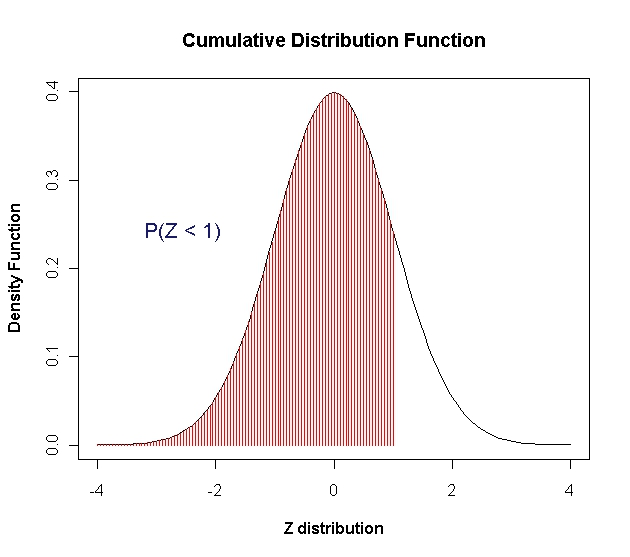
\includegraphics[scale=0.35]{images/6ACDF}

\end{center}
Cumulative Distribution Function $P(Z \leq 1)$.
\end{frame}

\end{document}
